\documentclass[addpoints,11pt]{exam}

\usepackage{alltt}
\usepackage[margin=1in]{geometry}   % set up margins
\usepackage[T1]{fontenc}
\usepackage[usenames,dvipsnames]{xcolor}
\usepackage{enumerate}              % fancy enumerate
\usepackage{amsmath}                % used for \eqref{} in this document
\usepackage{amsthm}
\theoremstyle{definition}
\newtheorem{exmp}{Example}[section]
\usepackage{verbatim}               % useful for \begin{comment} and \end{comment}
\usepackage{eurosym}                % used for euro symbol
\usepackage{caption} 
\usepackage{graphicx}
\graphicspath{{Figures/}}
\usepackage{subcaption}
\usepackage{color}
\usepackage{float}
\usepackage{amssymb}
\usepackage{sgamevar}
\usepackage{sgame}
\usepackage[colorlinks=true]{hyperref}
\hypersetup{colorlinks=true, citecolor=ForestGreen, linkcolor=BlueViolet, urlcolor=Magenta}

\usepackage{array}
\newcolumntype{H}{@{}>{\lrbox0}l<{\endlrbox}}


%Solutions or nah (blank next two lines out for no solutions, unblank #3)
%\printanswers
%\newcommand{\dd}[1]{\par {\textbf{\textcolor{red}{#1}}}}
\newcommand{\dd}[1]{}  


\setlength\parindent{0pt}
\unframedsolutions
\SolutionEmphasis{\color{red}}
\CorrectChoiceEmphasis{\color{red}}
\renewcommand{\choicelabel}{(\alph{choice})}
\newcommand{\blank}[0]{\underline{\hspace{3cm}}}
\pointformat{\bfseries[\thepoints]}
\pointpoints{pt}{pts}
\pointsinrightmargin

\begin{document}


\title{\textbf{Homework 1 \dd{Solutions}} \\ \vspace{2 mm} {\large ECON 101}}
\author{David A. D\'iaz}
\date{Summer I 2016
}
\maketitle

\makebox[\textwidth]{Name:\enspace\hrulefill}
\\

\makebox[\textwidth]{ONYEN:\enspace\hrulefill}
\\

\makebox[\textwidth]{PID:\enspace\hrulefill}
\\

\begin{center}
	\fbox{\fbox{\parbox{5.5in}{\centering
				This homework is due on \textbf{May 17} by \textbf{1PM}. Show work for all questions that require it (including multiple choice questions), attaching extra sheets as necessary. Multiple choice answers should be bubbled in on a scantron. For the short answer section, write legibly and make sure to box final answers. The total number of points available on this assignment is \textbf{100}.}}}
\end{center}

\subsection*{Multiple Choice [2 pts each]}

\begin{questions}
	
	\question A trade-off exists between a clean environment and a higher level of income in that 
		\begin{choices}
			\CorrectChoice laws that reduce pollution raise the costs of production and reduce incomes.
			\choice studies show that individuals with higher levels of income actually pollute less than low-income individuals.
			\choice efforts to reduce pollution are typically not successful.
			\choice by employing individuals to clean up pollution, employment and income both rise.
		\end{choices}
		
		\begin{solution}
			Choice (a) is the only one illustrating a trade-off.
		\end{solution}
	
	\question The following is a normative statement: ``By reducing financial constraints for poor individuals, the \textit{Prospera} poverty reduction program in Mexico causes more low-skilled immigrants to migrate to the US.''
	
		\begin{choices}
			\choice True
			\CorrectChoice False
		\end{choices} 
		
		\begin{solution}
			This is a positive statement. It is not making a value judgment and can be proved or disproved by examining data.
		\end{solution}
			
	\question Refer to Figure \ref{fig1}. If the economy moves from point A to point C, the opportunity cost is
		\begin{choices}
			\choice 10 toasters
			\CorrectChoice 20 toasters
			\choice 30 toasters
			\choice 30 toothbrushes
		\end{choices}
		
	\begin{figure}[H]
		\centering
		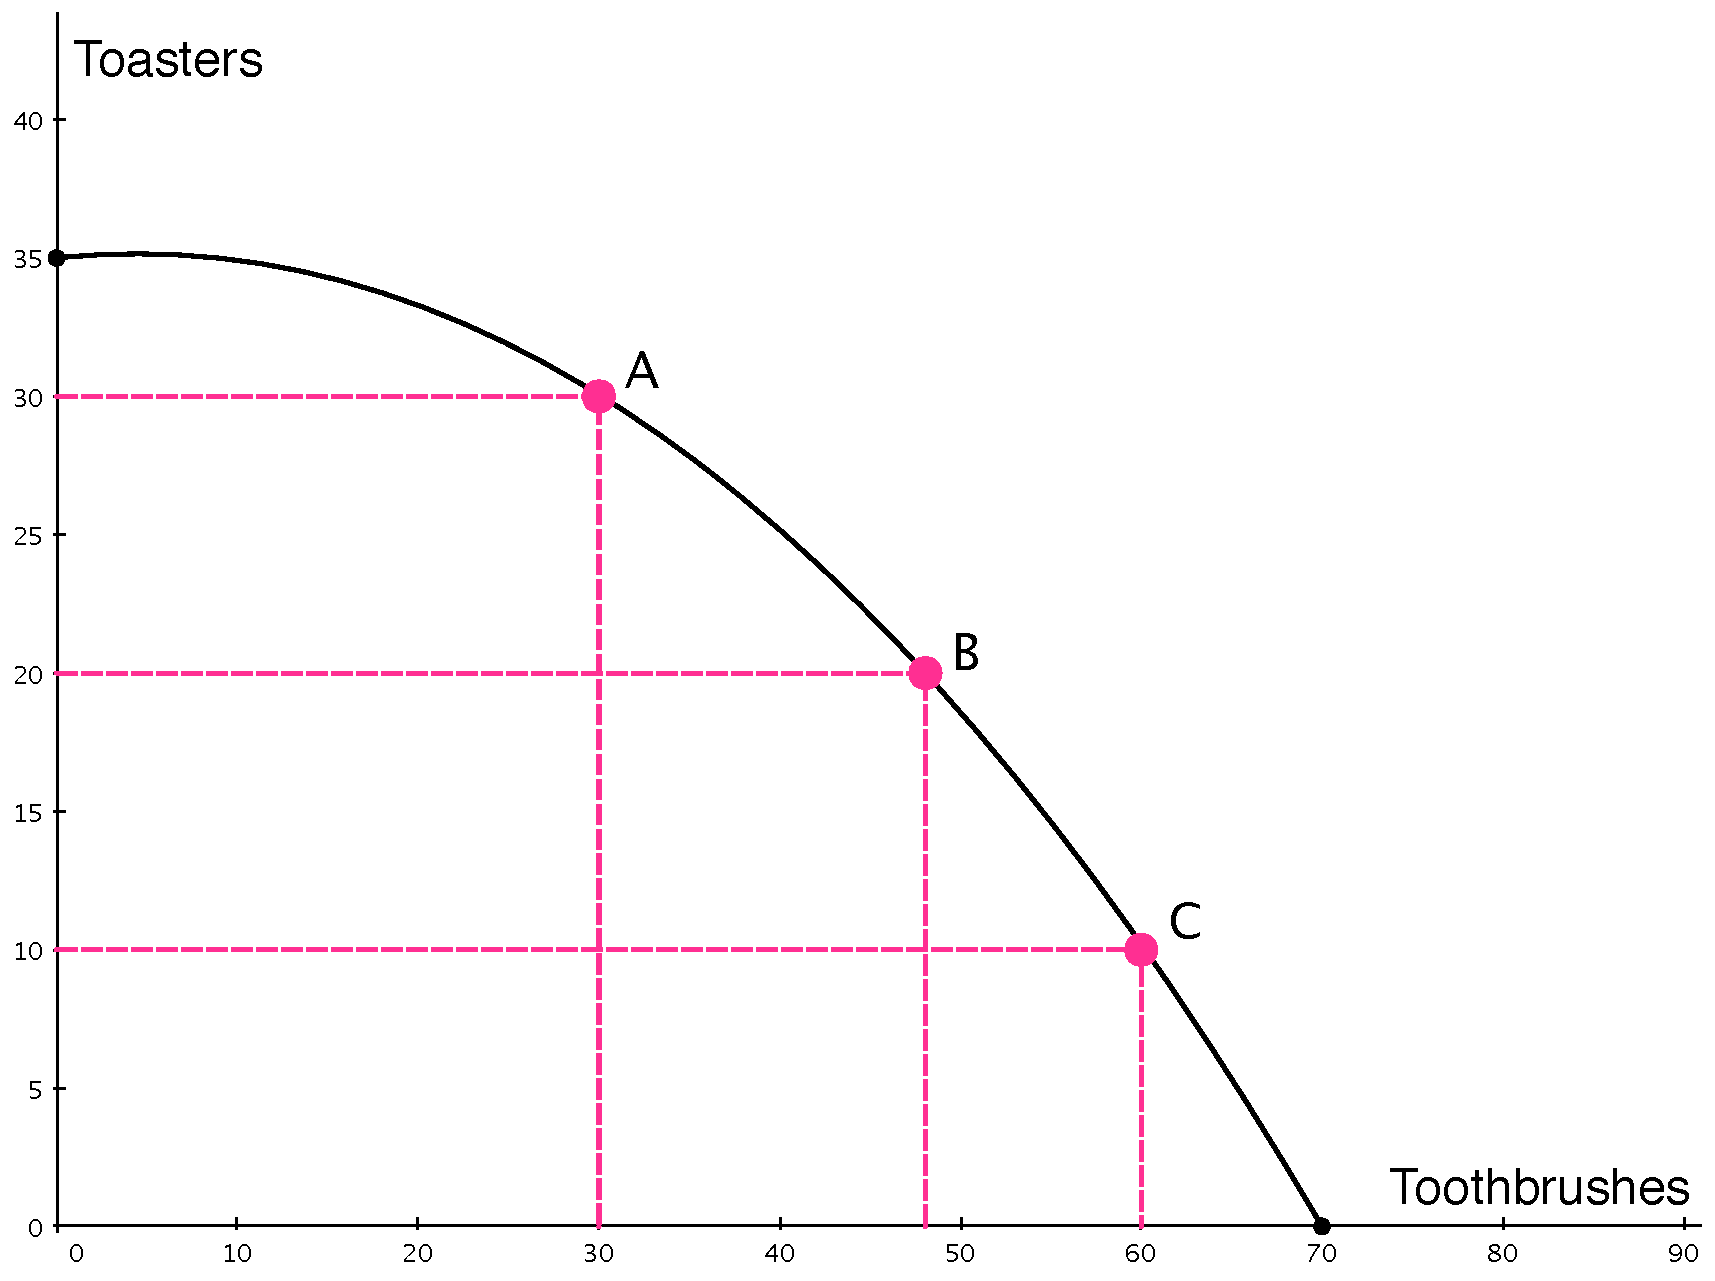
\includegraphics[scale=.3]{hw1_plot1.pdf}
		\caption{Production Possibilities Frontier}
		\label{fig1}
	\end{figure}
	
	\begin{solution}
		Moving from point A to point C yields a gain of 30 toothbrushes (30 $\rightarrow$ 60 brushes), but 20 toasters must be given up (30 $\rightarrow$ 10 toasters).
	\end{solution}
			
	\question Jackson spends an hour studying rather than playing soccer with his friends. The opportunity cost to him of studying is
		\begin{choices}
			\choice zero since Jackson chose to study rather than play soccer, the value of studying was higher to him than that of watching tv.
			\CorrectChoice the enjoyment he would have received from playing soccer with his friends.
			\choice the improvement in his grades from studying.
			\choice the improvement in his grades minus the benefits of playing soccer.
		\end{choices}
		
		\begin{solution}
			The OC of an activity is the value of the next best alternative.
		\end{solution}
		
	\question You won a free ticket to see a twenty one pilots concert (which has no resale value). Milky Chance is performing on the same night and is your next-best alternative activity. Tickets to see Milky Chance cost \$40. On any given day, you would be willing to pay up to \$50 to see Milky Chance. Assume there are no other costs of seeing either performer. Based on this information, what is the opportunity cost of seeing twenty one pilots?
		\begin{choices}
			\choice \$0
			\CorrectChoice \$10
			\choice \$40
			\choice \$50
		\end{choices}
		
		\begin{solution}
			The OC of seeing TOP is the value of the next best alternative. That is, it is what you are giving up when you go to the TOP concert. OC = cost of TOP (\$0) + value of Milky Chance (\$50) -- cost of Milky Chance (\$40) = \$10.
		\end{solution}
		
	\question Allie's Bakery makes fresh bread every morning at 6:00AM and throws out any remaining bread at closing time, 4:00PM. They sell the bread for \$3.00 a loaf and it costs them \$1.25 to make each one. Throwing away the bread is costless. The manager has 30 loafs of bread left over at 3:30PM today. Which of the following alternatives is most attractive?
		\begin{choices}
			\choice Lower the price of the remaining bread, but no lower than \$1.25.
			\CorrectChoice Lower the price of the remaining bread, even if it falls below \$1.25.
			\choice Throw the bread away now. No one wants it anyways.
			\choice Do nothing.
		\end{choices}
		
		\begin{solution}
			The cost of making the bread in the morning is a \underline{sunk cost}. You should sell the bread as long as MB $\ge$ MC. Since the MC of selling the bread is \$0, you should sell the bread for anything greater than \$0.
		\end{solution}
		
\newpage

		\question A person has a comparative advantage in activity $X$ when that person's
		\begin{choices}
			\choice opportunity cost of performing that activity is very high.
			\choice ability to perform that activity exceeds that all of other people.
			\choice government negotiates a favorable trade agreement.
			\CorrectChoice opportunity cost is lower than other trading partners.
		\end{choices}
		
		\begin{solution}
			See class notes.
		\end{solution}


\uplevel{For questions \ref{blah1} -\ref{blah2}, consider the following scenario: Two individuals, John and Yoko, own a garden with apple trees and berry bushes. Once a year they need to harvest their fruits. The following table shows how many berries and apples each can harvest per hour.}
		
\begin{table}[ht]
	\caption*{Berry and Apple Production}
	\centering
	\begin{tabular}{  c| c  c }        
		
		& Berries & Apples \\
		\hline
		John & 100 & 50 \\
		
		Yoko  & 200 & 75 \\
		
	\end{tabular}
\end{table}

	\question \label{blah1} Which of the following is true?
		\begin{choices}
			\choice Yoko has the absolute advantage in harvesting apples, and John has the absolute advantage in harvesting berries
			\choice John has the absolute advantage in harvesting apples, and Yoko has the absolute
			advantage in harvesting berries.
			\choice John has the absolute advantage in both harvesting apples and berries.
			\CorrectChoice Yoko has the absolute advantage in both harvesting apples and berries.
		\end{choices}
		
		\begin{solution}
			Yoko can produce more of both goods than John given the same number of inputs (one hour).
		\end{solution}
		
	\question John's opportunity cost of harvesting 10 apples is
		\begin{choices}
			\choice 100 berries
			\choice 50 berries
			\CorrectChoice 20 berries
			\choice 10 berries
		\end{choices}
		
		\begin{solution}
			100 berries : 50 apples $\rightarrow$ 20 berries : 10 apples.
		\end{solution}
		
	\question \label{blah2} If John and Yoko want to maximize their joint productivity,
		\begin{choices}
			\CorrectChoice John should harvest apples and Yoko should harvest berries.
			\choice Yoko should harvest apples and John should harvest berries.
			\choice John should harvest both, apples and berries.
			\choice Yoko should harvest both, apples and berries.
		\end{choices}
		
		\begin{solution}
			John: 100 berries : 50 apples $\Rightarrow$ 2 berries : 1 apple, 1 berry : .5 apples. 
		\\ Yoko: 200 berries : 75 apples $\Rightarrow$ 2.67 berries : 1 apple, 1 berry : .375 apples. John has a lower OC of producing apples than Yoko and so he has a CA in producing apples. Yoko has a CA in berries. To maximize productivity, each party will specialize in the good for which they have a CA.
		\end{solution}
				
		
\newpage
		
\uplevel{For questions \ref{blah3}-\ref{blah4}, refer to Figure \ref{MC18}, which shows the daily production possibilities of two brothers, Jony and Dany.}

		
		
		\begin{figure}[H]
			\centering
			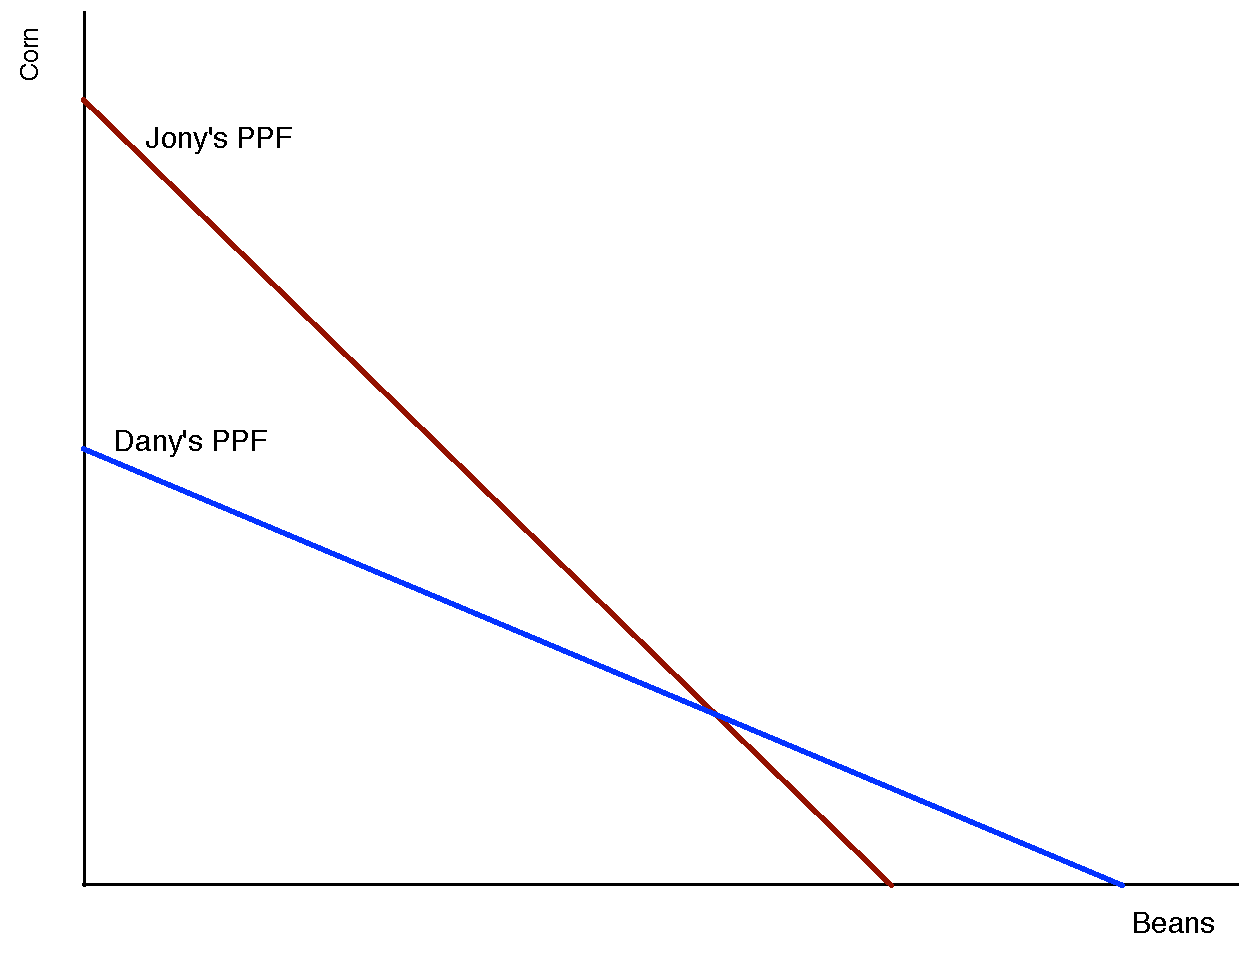
\includegraphics[scale=.4]{Final_MC18.pdf}
			\caption{Production of Beans and Corn}
			\label{MC18}
		\end{figure}
		

			
			\question \label{blah3} From their respective PPFs, we can conclude that
			
			\begin{choices}
				\CorrectChoice Dany has an absolute advantage in the production of beans, while Jony has an absolute advantage in the production of corn.
				\choice Dany has an absolute advantage in the production of both beans and corn.
				\choice Dany has an absolute advantage in the production of corn, while Jony has an absolute advantage in the production of beans.
				\choice Jony has an absolute advantage in the production of both beans and corn.
			\end{choices}
			
			\begin{solution}
				PPFs show max daily production for Jony and Dany. Jony can produce more corn in a day, while Dany can produce more beans.
			\end{solution}
			
			\question \label{blah4} Additionally, we can also say that 
			
			\begin{choices}
				\choice Jony has a comparative advantage in both goods, and Dany has a comparative advantage in neither good.
				\choice Jony has a comparative advantage in neither good, and Dany has a comparative advantage in both goods.
				\CorrectChoice Jony has a comparative advantage in corn, and Dany has a comparative advantage in beans.
				\choice Jony has a comparative advantage in beans, and Dany has a comparative advantage in corn.
				\choice None of the above. Not enough information given.
			\end{choices}
			
			\begin{solution}
				Slope of the PPFs gives the OC of the good on the x-axis. Steeper slope = higher OC of beans. The slope of Dany's PPF is less than Jony's, so Dany has a lower OC in producing beans $\Rightarrow$ Dany has CA in beans. OC of corn is reciprocal of the slope, so Jony has lower OC and thus CA in producing corn.
			\end{solution}
			
		
\newpage

\uplevel{Refer to Table \ref{MC8} for questions \ref{blah5}-\ref{blah6}, which shows the number of hours it takes Hank and George to produce one belt or shoe.}

\begin{table}[ht]
	\caption{Hours to produce 1 unit of}
	\centering
	\begin{tabular}{  c| c c} 
		
		& Belts & Shoes \\
		\hline
		Hank & 3 & 9 \\
		George & 12 & 12 \\
	\end{tabular}
	\label{MC8}
\end{table}



\question \label{blah5} A terms of trade where 1 shoe would be traded for 4 belts is proposed. Will the two parties agree to this price?

\begin{choices}
	\choice Yes. The terms of trade will make both parties better off.
	\choice No. The terms of trade will make George worse off.
	\CorrectChoice No. The terms of trade will make Hank worse off.
	\choice No. The terms of trade will make both parties worse off.
\end{choices}

\begin{solution}
	Hank: 1 belt/3 hours : 1 shoe/9 hours $\Rightarrow$ 1 belt : 1/3 shoe, 1 shoe : 3 belts. \\
	George: 1 shoe : 1 belt. \\
	Terms of trade have to be 1 shoe : $X$ belts, where $1<X<3$. \\
	George exports shoes to Hank in exchange for belts. \\
	If 1 shoe trades for 4 belts, Hank is worse off because he is giving up more belts for each shoe than if just he produced on his own. George would be better off because he would be getting more belts in exchange for a shoe than he could get on his own.
\end{solution}

\question \label{blah6} Which of the following terms of trade, if any, would make both Hank and George \textbf{strictly} better off?

\begin{choices}
	\choice 200 belts per 400 shoes
	\CorrectChoice 50 belts per 25 shoes
	\choice 100 shoes per 100 belts
	\choice 400 belts per 50 shoes
	\choice None of the above.
\end{choices}

	\begin{solution}
		Terms of trade in terms of shoes: 1 shoe : $X$ belts, where $1<X<3$. Check each option: \\
		(a) 200 belts : 400 shoes $\Rightarrow$ 1 shoe : 1/2 belt. \\
		(b) 50 belts : 25 shoes $\Rightarrow$ 1 shoe : 2 belts \\
		(c) 100 shoes : 100 belts $\Rightarrow$ 1 shoe : 1 belt \\
		(d) 400 belts : 50 shoes $\Rightarrow$ 1 shoe : 8 belts.
	\end{solution}

		
\question Suppose the market for iPods is initially in equilibrium, and the demand for iPods suddenly decreases. This decrease in demand will

\begin{choices}
	\choice cause a surplus of iPods at the original equilibrium price, and the price of iPods will increase to the new equilibrium level.
	\CorrectChoice cause a surplus of iPods at the original equilibrium price, and the price of iPods will decrease to the new equilibrium level.
	\choice cause a shortage of iPods at the original equilibrium price, and the price of iPods will increase to the new equilibrium level.
	\choice cause a shortage of iPods at the original equilibrium price, and the price of iPods will decrease to the new equilibrium level.
\end{choices}

\begin{solution}
	Demand shifts left, causing a surplus at the original equilibrium price. This puts downward pressure on prices and the new equilibrium price will be lower.
\end{solution}

\question If an economy goes into a recession and incomes fall, what happens in the markets for inferior goods?

\begin{choices}
	\CorrectChoice Equilibrium prices and quantities both rise.
	\choice Equilibrium prices and quantities both fall.
	\choice Equilibrium prices rise, quantities fall.
	\choice Equilibrium prices fall, quantities rise.
\end{choices}

\begin{solution}
	Demand for inferior goods will increase as incomes fall. An increase in demand will lead to a higher equilibrium price and quantity.
\end{solution}

\newpage

\question An increase in \blank will cause a movement along a given demand curve, which is called a change in \blank.

\begin{choices}
	\choice supply; demand
	\CorrectChoice supply; quantity demanded
	\choice demand; supply
	\choice demand; quantity supplied
\end{choices}

\begin{solution}
	A movement along the demand curve means that the demand curve stays fixed. The movement is caused by an shift (either an increase or decrease) in supply. A movement along a demand curve is called a change in quantity demanded.
\end{solution}

\question Which of the following might lead to an increase in the equilibrium price of grape jelly and a decrease in the equilibrium quantity of jelly sold?

\begin{choices}
	\choice An increase in the price of peanut butter (a complement to jelly).
	\choice An increase in the price of Marshmallow Fluff (a substitute for jelly).
	\CorrectChoice An increase in the price of grapes.
	\choice An increase in consumers' incomes (assume jelly is a normal good).
\end{choices}

\begin{solution}
	Going through each choice: \\
	(a) An increase in the price of a complement will decrease demand for jelly. This will cause a decrease in both the equilibrium price and quantity. \\
	(b) An increase in the price of a substitute will increase demand for jelly. This will cause an increase in both the equilibrium price and quantity. \\
	(c) An increase in the price of an input will cause a decrease in supply. This will lead to an increase in the equilibrium price of jelly and a decrease in equilibrium quantity. \\
	(d) An increase in income will lead to an increase in demand for jelly. Same effect as (b).
\end{solution}

	\question Consider the market for coffee ice cream in the US. There is currently a large strike of coffee bean pickers in Colombia, a major exporter of coffee beans. Given this, the equilibrium price of coffee ice cream in the US
	
	\begin{choices}
		\choice will increase, while the equilibrium quantity will increase.
		\choice will decrease, while the equilibrium quantity will increase.
		\CorrectChoice will increase, while the equilibrium quantity will decrease.
		\choice will decrease, while the equilibrium quantity will decrease.
	\end{choices}
	
	\begin{solution}
		The strike will lead to a decrease in the supply of coffee beans, increasing their price. This increase in coffee bean prices is seen as an increase in input prices for coffee ice cream producers, thus decreasing the supply of coffee ice cream. This will lead to an increase in the equilibrium price and a decrease in quantity in the market for coffee ice cream.
	\end{solution}
			
		\question Suppose the demand for single family homes increases due to a decline in interest rates. At the same time, a major home builder goes bankrupt and no longer builds homes. As a result, the equilibrium quantity of single family homes
		
		\begin{choices}
			\choice increases, while the equilibrium price of homes changes ambiguously.
			\CorrectChoice changes ambiguously, while the equilibrium price of homes increases.
			\choice changes ambiguously, while the equilibrium price of homes decreases.
			\choice decreases, while the equilibrium price of homes changes ambiguously.
			\choice None of the above.
		\end{choices}
		
	\begin{solution}
		Increase in demand increases the equilibrium price and quantity. Decrease in supply increases the equilibrium price and decreases quantity. The equilibrium price will increase, but effect on equilibrium quantity is ambiguous.
	\end{solution}
	
	\question Suppose that the price of coffee, a complement to donuts, decreases. As a result, the equilibrium price of donuts \blank and total surplus in the donut market \blank.
	
	\begin{choices}
		\CorrectChoice increases; increases
		\choice increases; decreases
		\choice decreases; decreases
		\choice decreases; increases
	\end{choices}
	
	\begin{solution}
		A decrease in the price of a complement will increase demand for donuts. This will increase the equilibrium price and quantity. Total surplus will increase.
	\end{solution}

	
	\uplevel{For questions \ref{blah7}-\ref{blah8}, refer to Figure \ref{MC1} below, which shows demand curves relating to some inferior good $A$.}
	
	\begin{figure}[H]
		\centering
		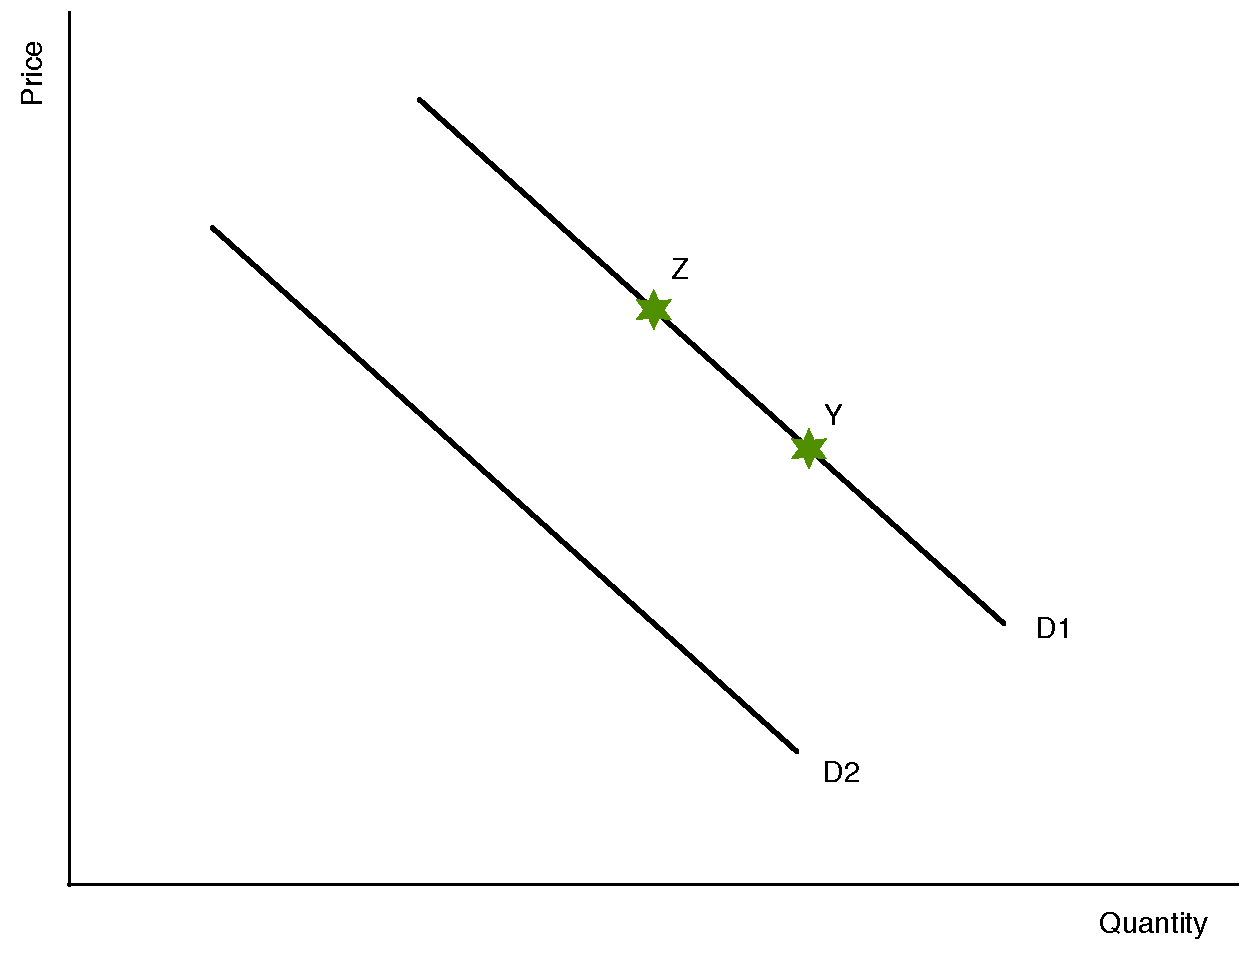
\includegraphics[scale=.38]{Exam1_MC2.pdf}
		\caption{Demand for Good $A$}
		\label{MC1}
	\end{figure}
	
		
		\question \label{blah7} There is some other good $B$ that is complements with good $A$. All else equal, a decrease in the price of good $B$ would cause a move from  
		
		\begin{choices}
			\CorrectChoice D2 to D1.
			\choice Y to Z.
			\choice Z to Y.
			\choice D1 to D2.
		\end{choices}
		
		\begin{solution}
			A decrease in the price of a complement will increase demand for good $A$.
		\end{solution}
		
		
		\question \label{blah8} All else equal, an increase in the price of good $A$ would cause a move from
		
		\begin{choices}
			\choice D2 to D1.
			\CorrectChoice Y to Z.
			\choice Z to Y.
			\choice D1 to D2.
		\end{choices}
		
		\begin{solution}
			An increase in the price of good $A$ will cause a movement along the demand curve.
		\end{solution}
		
	
	\question Jen values her time at \$60 an hour. She spends 2 hours giving Collen a massage. Collen was willing to pay \$300 for the massage, but they negotiate a price of \$200. In this transaction,
	
	\begin{choices}
		\CorrectChoice consumer surplus is \$20 larger than producer surplus.
		\choice consumer surplus is \$40 larger than producer surplus.
		\choice producer surplus is \$20 larger than consumer surplus.
		\choice producer surplus is \$40 larger than consumer surplus.
	\end{choices}
	
	\begin{solution}
		Collen's WTP = \$300, while Jen's cost = \$60/hr $\times$ 2 = \$120. With $P$ = \$200, WTP = \$300 - \$200 = \$100 and PS = \$200 - \$120 = \$80.
	\end{solution}

\newpage

	\question Refer to Table \ref{wtp}, which gives the willingness to pay for 1 lb of kale of four individuals.
	
	\begin{table}[H]
		\caption{WTP for 1 lb Kale}
		\label{wtp}
		\centering
		\begin{tabular}{  c| c    }    
			
			Buyer   & WTP \\
			\hline
			Natalie & \$3.00 \\
			Avery & \$1.50 \\
			Meredith & \$5.00 \\
			Madi & \$.50 \\
		\end{tabular}
		
	\end{table} 
	
	If the market price for kale is \$1.50, the total consumer surplus realized is
	
	\begin{choices}
		\choice \$1.00.
		\choice \$1.50.
		\choice \$4.00.
		\CorrectChoice \$5.00.
	\end{choices}
	
	\begin{solution}
		$CS = WTP - P$. Natalie realizes $CS = \$1.50$, Avery realizes $CS = \$0$, and Meredith realizes $CS = \$3.50$. Madi does not buy the Kale because she's not willing to pay more than \$.50, and so her $CS = \$0$. Total $CS = \$5.00$.
	\end{solution}
	


	
	\question Producing a quantity larger than the equilibrium of supply and demand is inefficient because the marginal buyer's willingness to pay is
	
	\begin{choices}
		\choice negative.
		\choice zero.
		\CorrectChoice positive but less than the marginal seller's cost.
		\choice positive and greater than the marginal seller's cost.
	\end{choices}
	
	\begin{solution}
		TS = Buyer value - Seller cost. For $Q>Q^*$, the seller cost is greater than the buyer value (but both are still positive) and thus TS is reduced.
	\end{solution}


	\question Suppose demand for pizza shifts such that the market price for pizzas increases. Which of the following statements must be true?
	
	\begin{enumerate}[i.]
		\item Producer surplus increases as existing sellers in the market receive higher prices on the pizzas they were already selling.
		\item New sellers enter the market as a result of the price increase and realize surplus.
		\item Consumer surplus decreases due to the higher price of pizza.
	\end{enumerate}
	
	\begin{choices}
		\choice i and iii
		\CorrectChoice i and ii
		\choice ii and iii
		\choice i, ii, and iii
	\end{choices}
	
	\begin{solution}
		An increase in demand will lead to a higher market price and equilibrium quantity. This will increase producer surplus for both existing and new sellers in the market. $CS$ could potentially increase since $WTP$ increases at each quantity and there are more transactions taking place.
	\end{solution}
	
\newpage
	
	\question Figure \ref{MC23} shows the demand curve for Fanta.
		
		\begin{figure}[H]
			\centering
			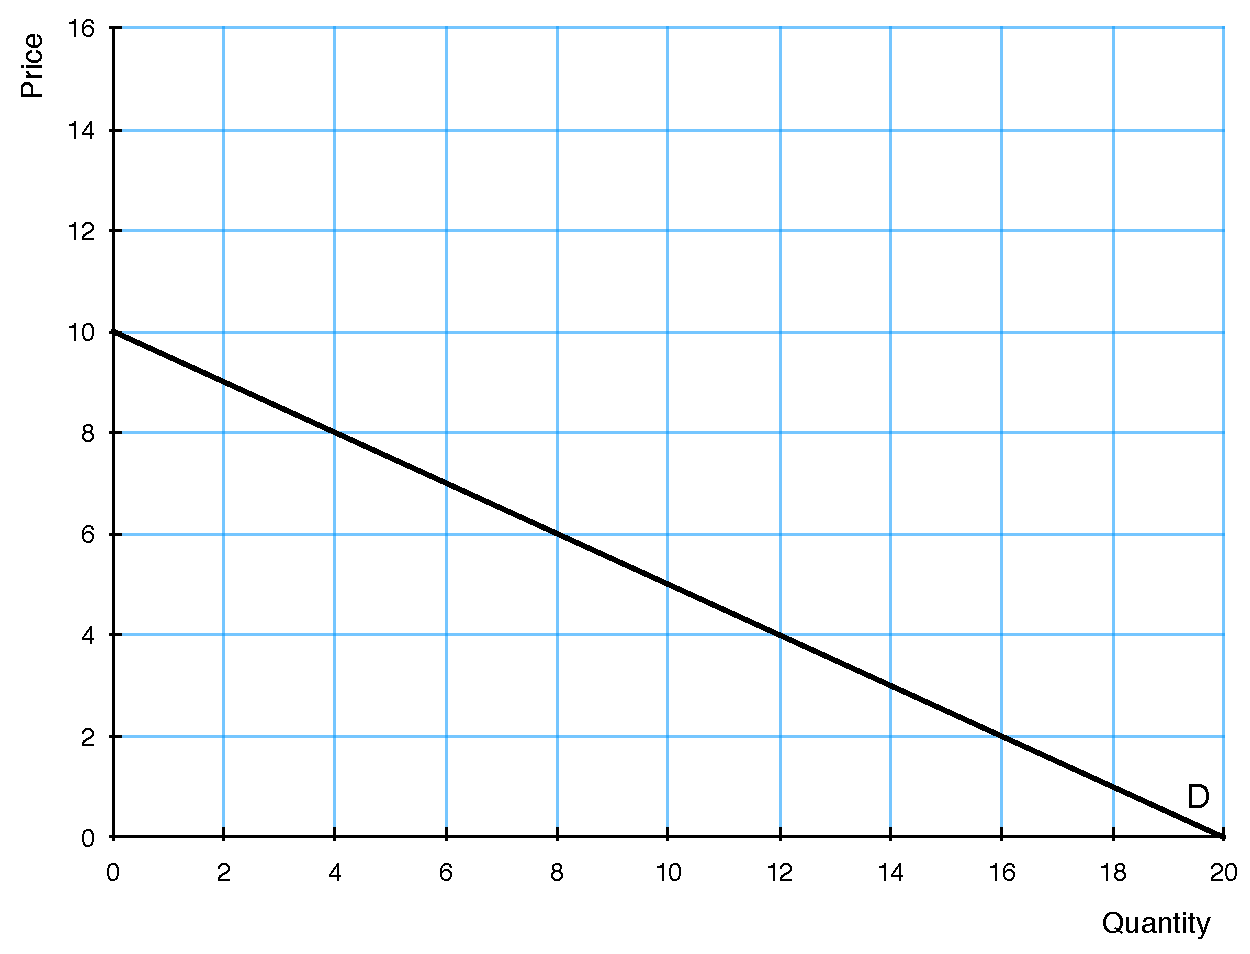
\includegraphics[scale=.45]{Exam1_MC22.pdf}
			\caption{Demand for Fanta}
			\label{MC23}
		\end{figure}
		
		If the price of Fanta decreases from \$8 to \$4, the increase in consumer surplus that is realized by \textbf{new buyers} entering the market due to the price decrease is 
		
		\begin{choices}
			\choice \$36.
			\choice \$32.
			\CorrectChoice \$16.
			\choice \$8.
		\end{choices}	
		
		\begin{solution}
			At $P=8,$ $Q_D = 4.$ At $P = 4,$ $Q_D = 12.$ New buyers realized the increase in surplus from $Q_D = 4$ to $Q_D = 12 = (1/2)\cdot4\cdot8=\$16.$
		\end{solution}


		
\uplevel{For questions \ref{blah9}-\ref{blah10}, consider Figure \ref{MC25}.}
		
		\begin{figure}[H]
			\centering
			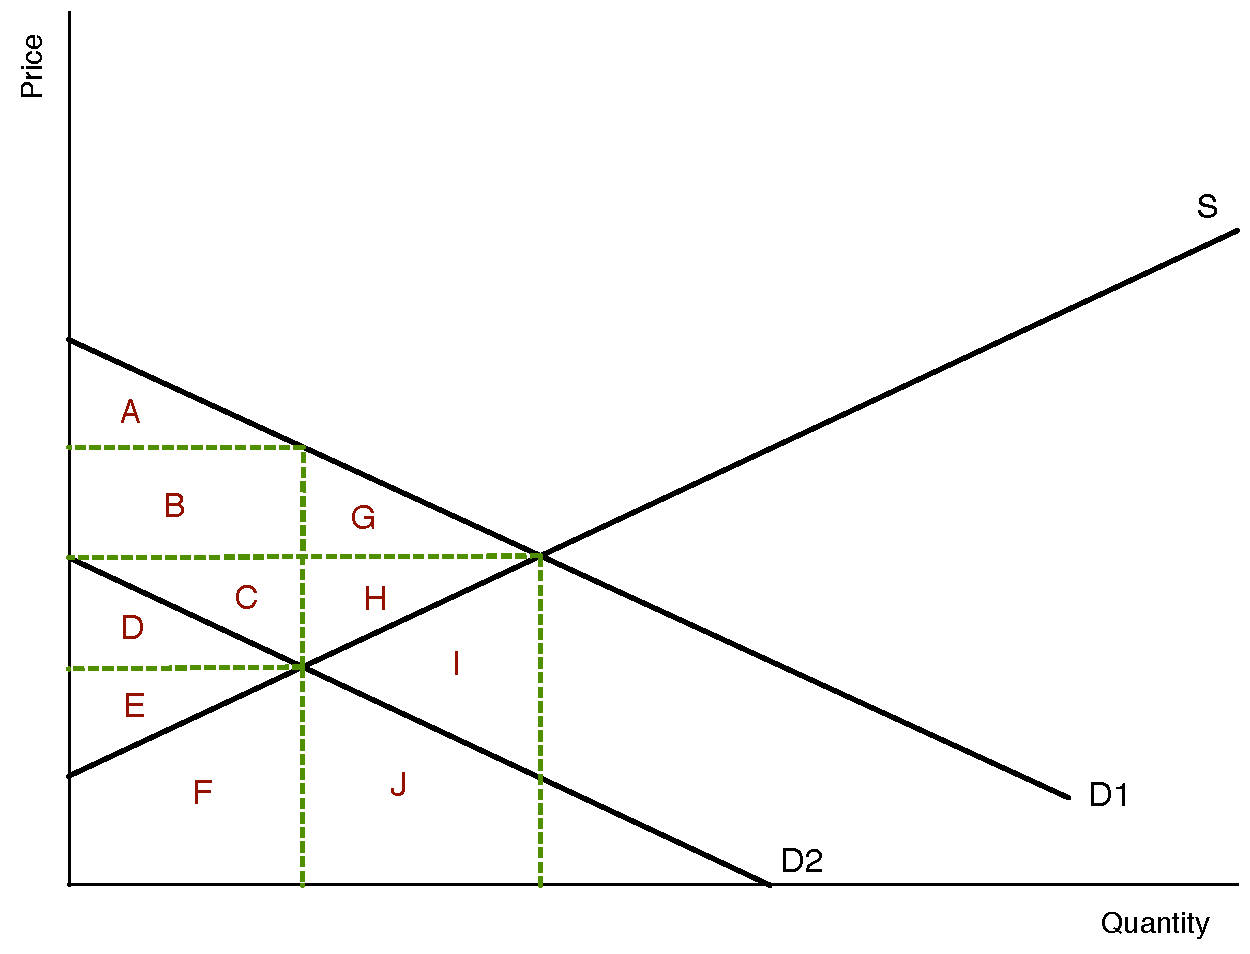
\includegraphics[scale=.45]{Exam1_MC25.pdf}
			\caption{Market for Fanta}
			\label{MC25}
		\end{figure}


		\question \label{blah9} If demand is originally given by D2, and then shifts to D1, total surplus in the market
		
		\begin{choices}
			\choice increases by areas A+B+C+G+H+I.
			\choice increase by areas A+B+C+D+E+G+H.
			\choice increases by areas A+B+C+D+E.
			\CorrectChoice increases by areas A+B+C+G+H.
			\choice None of the above.
		\end{choices}
		
		\begin{solution}
			$TS_0 = D+E.$ $TS_1 = D + E + A + B + C  + G + H$.
		\end{solution}
		
		\question \label{blah10} As a result of the increase in demand, producer surplus in the market 
			
			\begin{choices}
					\choice decreases by areas C+H.
					\CorrectChoice increases by areas D+C+H.
					\choice increases by areas E+D+C+H.
					\choice decreases by areas E+D.
					\choice None of the above.
				\end{choices}
				
		\begin{solution}
			$PS_0 = E.$ $PS_1 = E + D + C + H$.
		\end{solution}
		
\end{questions}

\subsection*{Short Answer}

\begin{questions}
	
	\question[3] Give three examples of trade-offs (that we have not discussed) you face in your life. 

	
	\question Imagine a society that produces military goods and consumption goods (``guns'' and ``butter'').
		\begin{parts}
			\part[4] Draw a production possibilities frontier for guns and butter. Label your plot clearly and use it for the remainder of this problem. Explain why it most likely has a bowed out shape. 
			
			\begin{solution}
				See Figure \ref{fig2} below. The PPF is ``bowed out'' due to the specialization of resources. Some resources are more suited to producing national defense while others are better suited to producing consumption goods. This leads to increasing opportunity costs as more of either good is produced.
			\end{solution}
			
			\part[2] Show a point that is impossible for the economy to achieve. Show a point that is feasible, but inefficient.
			
			\begin{solution}
				Any point outside of the PPF is impossible to achieve. Points strictly inside the PPF are feasible, but inefficient as more can be produced given the society's resources.
			\end{solution}
			
			\part[2] Imagine that the society has two political parties. Hawks favor a strong military and Doves favor a small military. Show a point on the frontier that the Hawks might choose and a point the Doves might choose. 
			
			\begin{solution}
				Point H0 might be point the Hawks favor, while D0 would be one the Doves prefer.
			\end{solution}
			
			\part[4] Imagine an aggressive neighboring country reduces the size of its military. As a result, both the Hawks and Doves reduce their desired production of guns by the same amount. Which party would get the bigger ``peace dividend,'' measured by the increase in butter production? Explain why. \textbf{Hint:} Use your plot.
			
					
		\begin{solution}
			The Hawks and Doves both reduce their gun production by the same amount (H0 $\rightarrow$ H1 and D0 $\rightarrow$ D1, respectively). Due to increasing opportunity costs, the Hawks would see a much larger increase in butter production and thus would get the bigger ``peace dividend.''
			
				\begin{figure}[H]
							\centering
							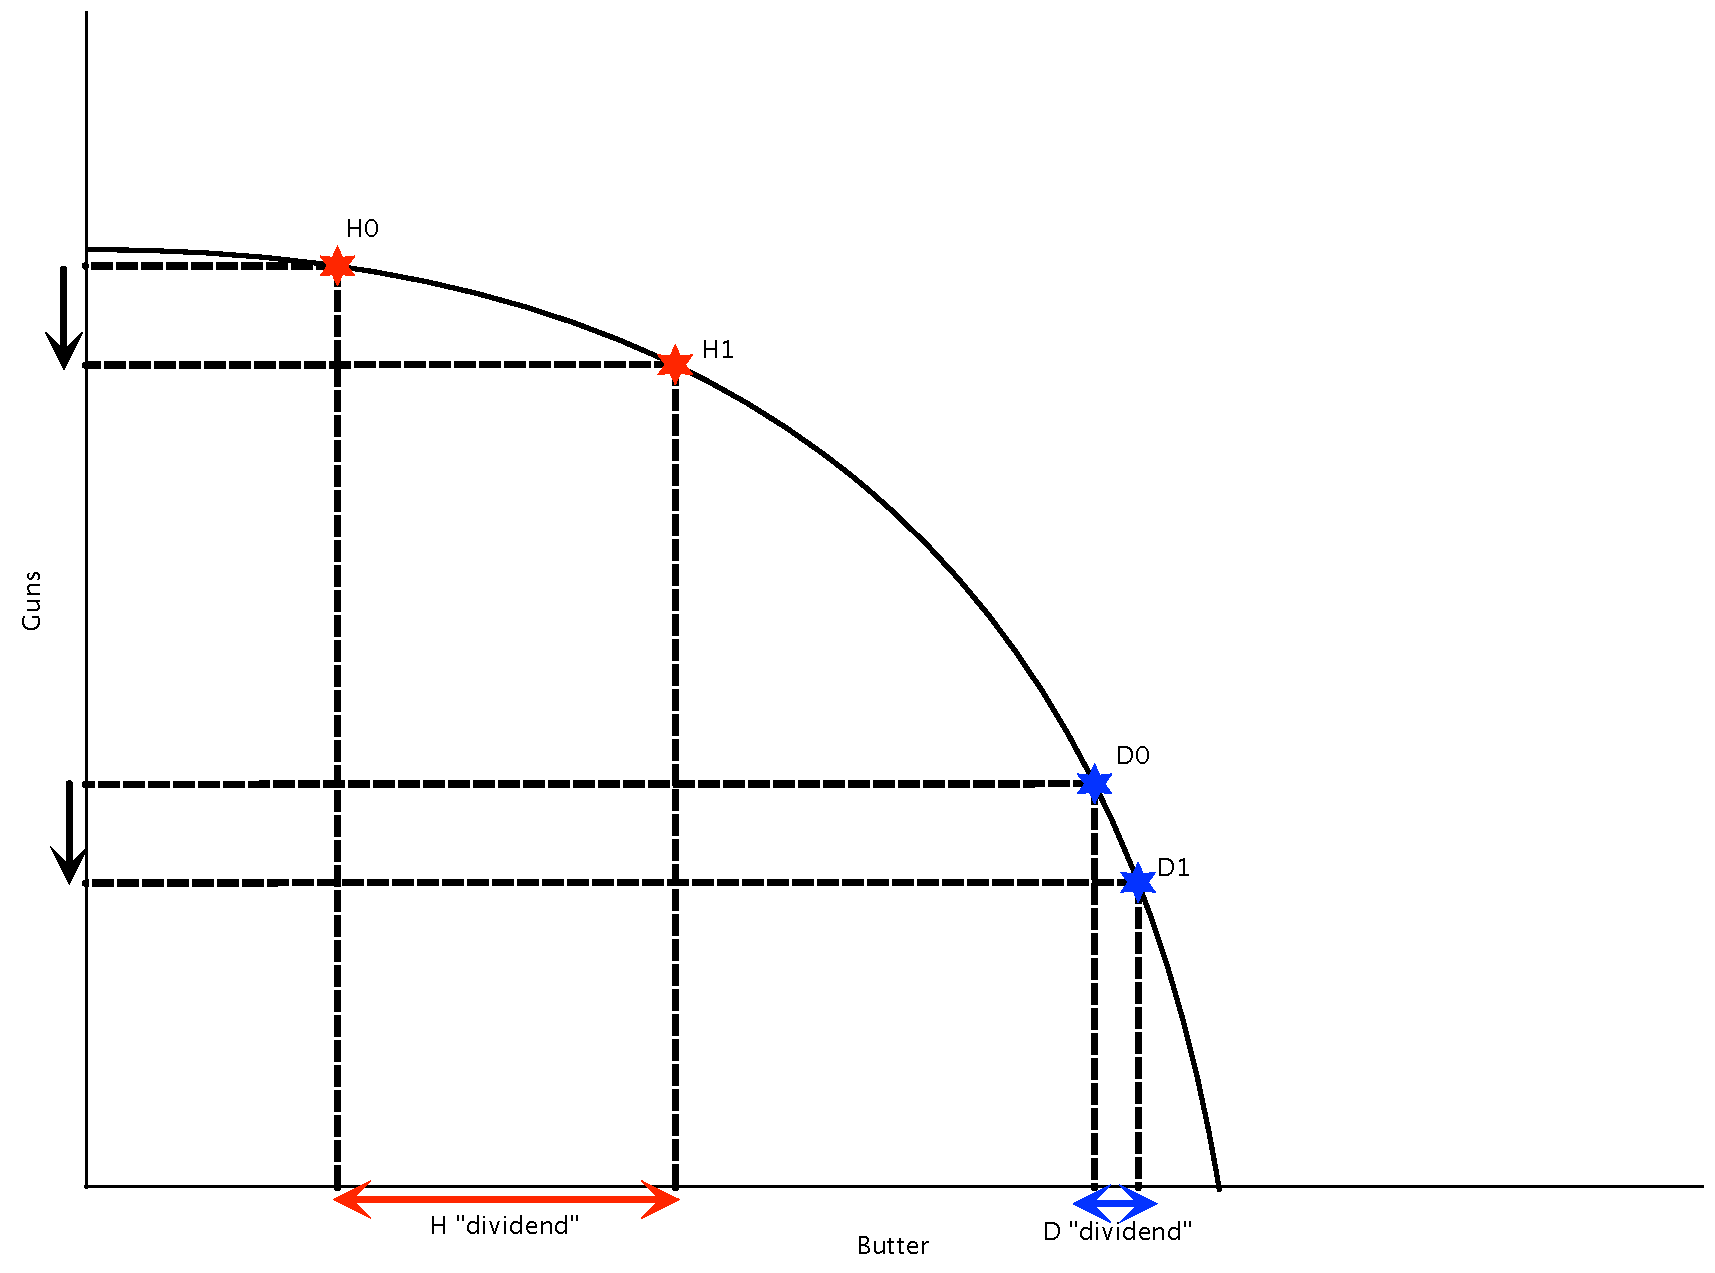
\includegraphics[scale=.38]{hw1_ppf.pdf}
							\caption{Production Possibilities Frontiers: Guns and butter}
							\label{fig2}
							
				\end{figure}
				
		\end{solution}
			
		\end{parts}
		
\newpage
		
	\question Argentina and Brazil can produce mangoes and bananas daily as given by the production possibilities frontiers in Figure \ref{fig3}. 
	
		\begin{figure}[H]
			\centering
			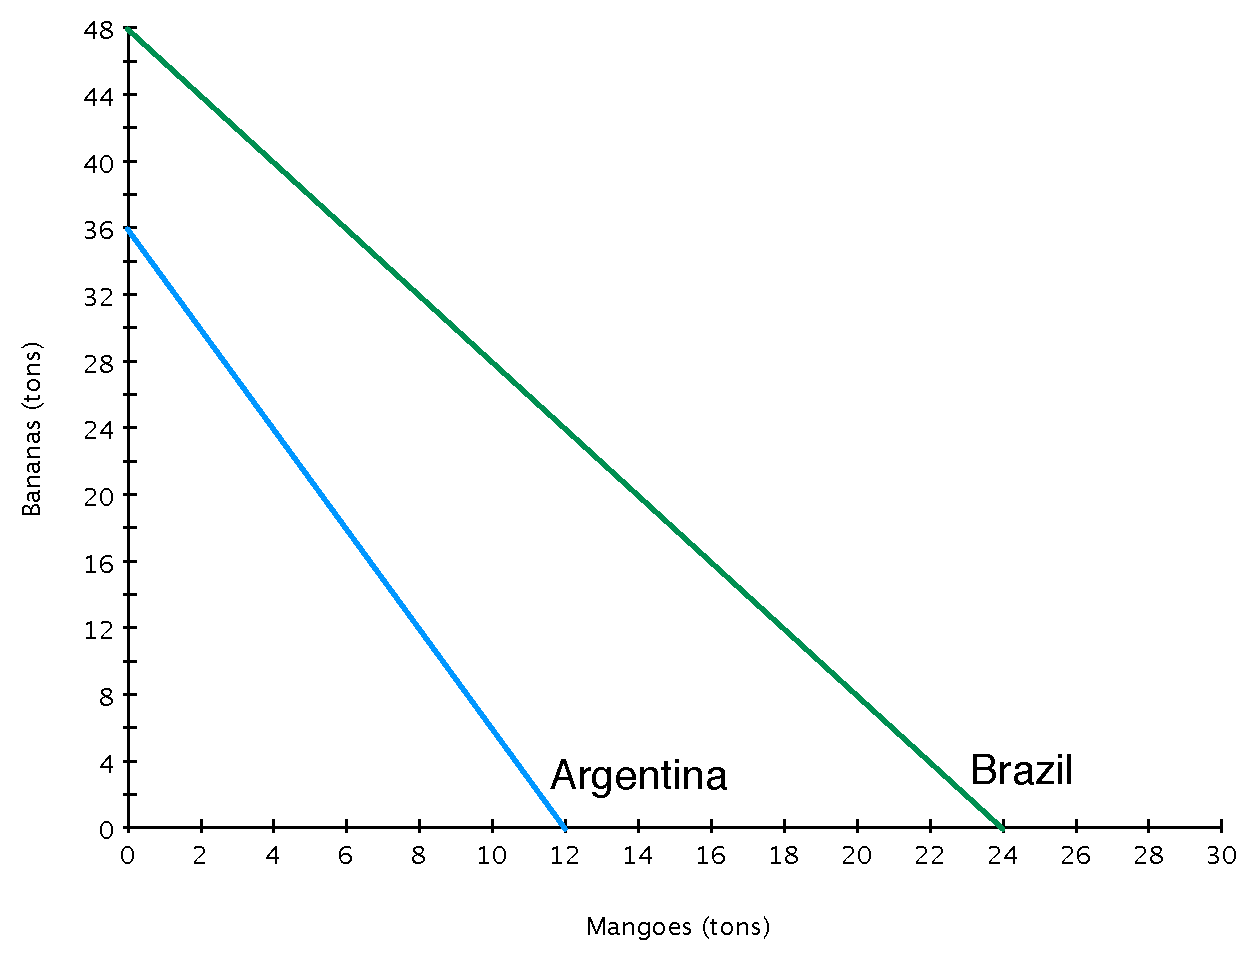
\includegraphics[scale=.36]{hw1_plot2.pdf}
			\caption{Production Possibilities Frontiers: ARG \& BRA}
			\label{fig3}
		\end{figure}
	
		\begin{parts}
			\part[2] Which country has an absolute advantage in bananas? In mangoes?
			
			\begin{solution}
				Brazil has an absolute advantage in producing both goods since their daily production of mangoes and bananas is greater than Argentina's.
			\end{solution}
			
			\part[5] For each country, determine the opportunity cost of 1 ton of bananas and 1 ton of mangoes. Which country has a comparative advantage in bananas? In mangoes? Given this, what are the expected trade patterns between the two countries? 
			
			\begin{solution}
				For each country, the opportunity cost of mangoes (the good on the x-axis) is the slope of their PPF. For Argentina, the slope is $36/12 = 3$ and for Brazil it is $48/24 = 2$. Thus, the OC of 1 mango is 3 bananas for Argentina and 2 bananas for Brazil. The OC of 1 banana is the reciprocal: 1/3 mango for Argentina and 1/2 mango for Brazil. Brazil has the CA in mangoes and Argentina has the CA in bananas. Brazil would export mangoes to Argentina in exchange for bananas.
			\end{solution}
						
			\part[2] Each country specializes in the good for which they have a comparative advantage. Give a terms of trade these countries might agree on in terms of \textit{mangoes}. That is, give a terms of trade in the form of 1 mango: $X$ bananas. 
			
			\begin{solution}
				In order for both countries to both be better off, the terms of trade must lie between the opportunity costs of mangoes for both countries. Then, the terms of trade must be 1 mango : $X$ bananas, where $2<X<3$. Looking at it from each country's perspective: \\ \\
			Brazil: Exports mangoes to Argentina. On their own, they could produce 2 bananas for each mango they give up. So, they must receive more than 2 bananas for each mango they export in order to be better off. \\ \\
			Argentina: Imports mangoes from Brazil. On their own, they give up 3 bananas for each mango they produce. So, must give up less than 3 bananas for each mango they import in order to be better off.
			\end{solution}
			
		\end{parts}
		
	\question[4] Suppose you are studying for your first economics exam with a classmate enrolled in a different section of 101 and they state the following: ``A decrease in the number of sellers might seem to increase the price of a good to consumers. But this increase in prices will decrease demand for the good, and this decrease in demand will send the price down again. So, in the end, we don't know for sure that a decrease in sellers will increase the price of the good.'' 
		
		Do you agree or disagree with their statement? Why or why not? 
		
		\begin{solution}
			Disagree. A decrease in the number of sellers will cause supply to shift left, which will increase the equilibrium price and decrease the equilibrium quantity. Demand will not change, but rather this shift in supply will cause a movement along the demand curve as quantity demanded decreases in response to the higher price.
		\end{solution}
	
	\question Table \ref{laptops} shows the willingness to pay and costs of eight buyers and sellers in the market for laptops. Each buyer would like to buy one laptop and each seller has one laptop to sell. Use the table to answer the following questions.
	\\
	
	\begin{table}[H]
		\caption{WTP and Seller Costs for Laptops}
		\label{laptops}
		\centering
		%c's to H's and vice-versa for HW Solutions
		\begin{tabular}{HH c|c|c|c|c}        
			
			WTP   & Seller Costs & WTP & SC & CS & PS & TS \\
			\hline
			\$175 & \$160 & \$175 & \$45 & \$50 & \$80 & \$130 \\
			\$155 & \$45 & \$155 & \$70 & \$30 & \$55 & \$85\\
			\$130 & \$140& \$150 & \$100 & \$25 & \$25 & \$50\\
			\$150 & \$200& \$130 & \$110 & \$5 & \$15 & \$20\\
			\$110 & \$110 & \textcolor{red}{\$125} & \textcolor{red}{\$125} & \$0 & \$0 & \$0 \\
			\$115 & \$100& \$115 & \$140 & ---\ & --- & ---\\
			\$125 & \$70& \$110 & \$160 & --- & --- & ---\\
			\$100 & \$125& \$100 & \$200 & --- & --- & ---\\
			
		\end{tabular}
	\end{table}
	
	
	\begin{parts}
		\part[3] If the market price is currently \$150, is there a shortage or a surplus? What do you expect will happen to the market price?
		
		\begin{solution}
			With a price of \$150, buyers who are willing to pay more than \$150 for a laptop would purchase one and sellers with a cost lower than \$150 would sell one. $Q_D =3$ and $Q_S = 6$. This price causes a surplus, so the market price will decrease.
		\end{solution}
		
		\part[3] If instead the market price was \$115, would there be a shortage or a surplus? What do you expect will happen to the market price? 
		
		\begin{solution}
			With a price of \$115, buyers who are willing to pay more than \$115 for a laptop would purchase one and sellers with a cost lower than \$115 would sell one. So, $Q_D =6$ and $Q_S = 4$. This price causes a shortage, so the market price will increase.
		\end{solution}
		
		\part[2] What is the equilibrium quantity and price in this market? 
		
		\begin{solution}
			At the equilibrium price, $Q_D = Q_S$ and WTP = seller cost = $P^*$ at this quantity. 
		\\\\
		Order the demand and supply schedules like in example from class: \\(1) WTP in descending order \& (2) Seller cost in ascending order. \\ Find where WTP = Seller cost.
		\\
		WTP = seller cost at the fifth transaction (5$^{th}$ row). This is the equilibrium quantity. The equilibrium price is equal to the WTP and seller cost at this transaction, $P^*=\$125.$
		\end{solution}
		
		\part[4] What is the value of consumer, producer, and total surplus at the equilibrium price? Could we increase total surplus by raising or lowering the price? 
		
			\begin{solution}
				$CS = WTP - P$, $PS = P - SC$ and $TS = CS + PS$ for each transaction that takes place. Adding the CS, PS, and TS from each transaction, consumer surplus in the market is \$110, producer surplus is \$175, and total surplus is  \$285. TS is maximized at the equilibrium price.
			\end{solution}
		
		
	\end{parts}
	
		\question What topics or questions gave you the most trouble on this homework assignment or the class material it encompassed? 

\end{questions}


\end{document}